% arara: lualatex: { shell: yes, interaction: nonstopmode }
\documentclass[10pt,a4paper]{article}
\input{layouts_origin/use}                 % 宏包导入
\input{layouts_origin/set_code}            % 样式设置 : codefence 相关包 : tcolorbox , minted , fcextra , fancyvrb
% \input{layouts_origin/set_call}          % 样式设置 : callout   tcolorbox

% ---- 启用数学堆叠
\stackMath
% ---- 常用简写
\let\xpndaft=\expandafter
\let\ncm=\newcommand
\let\rcm=\renewcommand
% ----- 排版相关
\newcommand{\cfbox}[2][blue]{%
  \setlength{\fboxsep}{0pt}%
  \setlength{\fboxrule}{0.4pt}%
  \colorlet{currentcolor}{.}%
  {\color{#1}%
  \fbox{\color{currentcolor}\ensuremath{#2}}}%
}
\let\ph=\phantom
\let\hph=\hphantom
\let\vph=\vphantom
\let\mrel=\mathrel
\let\mbin=\mathbin
\let\mop=\mathop
\let\mllap=\mathllap                 % 根据文本右侧对齐
\let\mrlap=\mathrlap                 % 根据文本左侧对齐
\let\mclap=\mathclap                 % 根据文本中央对齐
\def\vts#1{\lvert#1\rvert}
\def\prs#1{\left(#1\right)}
\def\bcs#1{\left\{#1\right\}}
\def\bks#1{\left[#1\right]}
\def\plr#1{\vph{(fg)}\smash{#1}}     % 柱子
\def\etc{\plr{\rm etc}}              % 省略号
\def\occ{\plr{\texttt{\_}}}          % 占位符
% ----- 变量注册模板 带高亮
% \def\gobble#1{}                      % 吞掉参数
\makeatletter
\def\RegistVarType#1{
  \@ifnextchar [%
  {\RegistVarType@{#1}}
  {\RegistVarType@{#1}[]}
}
\def\RegistVarType@#1[#2]{
  \xpndaft\def\csname var#1colorBG\endcsname{}
  \xpndaft\def\csname var#1font\endcsname{}
  \pgfkeys{%
    /var #1/.is family, /var #1,
    colorBG/.store in/.expand once = \csname var#1colorBG\endcsname,
    font/.store in/.expand once = \csname var#1font\endcsname,
    #2
  }
  \xpndaft\def\csname var#1\endcsname##1{%
    \setlength{\fboxsep}{0pt}%
    \setlength{\fboxrule}{0pt}%
    \let\RegistVar@Cache=\relax  
    \xpndaft\ifx\csname var#1colorBG\endcsname\empty
      \def\RegistVar@Cache{\fbox}%
    \else
      \def\RegistVar@Cache{\colorbox{\csname var#1colorBG\endcsname}}%
    \fi
    \RegistVar@Cache{\ensuremath{\plr{\csname var#1font\endcsname ##1}}}%
  }
}
% ------ 常用变量注册模板 带高亮
\def\RegistVarFamily#1Type#2{
  \@ifnextchar D%
  {\RegistVarFamily@{#1}{#2}}
  {\RegistVarFamily@{#1}{#2}Disp{#1}}
}
\def\RegistVarFamily@#1#2Disp#3{%
  \xpndaft\def\csname #2#1\endcsname{%
    \csname var#2\endcsname{{#3}^{}}%
  }
  \xpndaft\def\csname #2#1n\endcsname##1{%
    \csname var#2\endcsname{{#3}_{##1}^{}}%
  }
  \@ifnextchar p
  {\RegistVarFamily@Loop{#1}{#2}{p}{'}{#3}}
  {\relax}
}
\def\RegistVarFamily@Loop#1#2#3#4#5p{% 
  \xpndaft\def\csname #2#1#3\endcsname{%
    \csname var#2\endcsname{{#5}#4}%
  }
  \xpndaft\def\csname #2#1#3n\endcsname##1{%
    \csname var#2\endcsname{{#5}#4_{##1}}%
  } 
  \@ifnextchar p
  {\RegistVarFamily@Loop{#1}{#2}{#3p}{#4'}{#5}} 
  {\relax}   
}
\makeatother
\makeatletter
% ----- 运算符注册模板
\def\RegistOpr#1Type{
   \@ifnextchar A%
  {\RegistOpr@TypeA@{#1}} % 发现 A,交给 TypeA 处理
  {\@ifnextchar B%
  {\RegistOpr@TypeB@{#1}} % 发现 B,交给 TypeB 处理
  {\@ifnextchar C%
  {\RegistOpr@TypeC@{#1}} % 发现 C,交给 TypeC 处理
  {\@ifnextchar D%
  {\RegistOpr@TypeD@{#1}} % 发现 D,交给 TypeD 处理
  {\relax}}}}
}
\def\RegistOpr@TypeA@#1A{
  \@ifnextchar [%
  {\RegistOpr@TypeA@opt{#1}}
  {\RegistOpr@TypeA@opt{#1}[]}
}
\def\RegistOpr@TypeB@#1B{
  \@ifnextchar [%
  {\RegistOpr@TypeB@opt{#1}}
  {\RegistOpr@TypeB@opt{#1}[]}
}
\def\RegistOpr@TypeC@#1C{
  \@ifnextchar [%
  {\RegistOpr@TypeC@opt{#1}}
  {\RegistOpr@TypeC@opt{#1}[]}
}
\def\RegistOpr@TypeD@#1D{
  \@ifnextchar [%
  {\RegistOpr@TypeD@opt{#1}}
  {\RegistOpr@TypeD@opt{#1}[]}
}
\def\RegistOpr@TypeA@opt#1[#2]{
  \ExpandArgs{c}\def{opr#1defaultType}{}
  \ExpandArgs{c}\def{opr#1display}{}
  \pgfkeys{
    /opr/typeA/#1/.is family, /opr/typeA/#1,
    default type/.store in/.expand once = \csname opr#1defaultType\endcsname,
    display as/.store in/.expand once = \csname opr#1display\endcsname,
    #2
  }
  \ExpandArgs{c}\DeclareDocumentCommand{#1}{%
    +O{\UseName{opr#1defaultType}}%
  }{%
    \plr{\ensuremath{%
      \stackunder[0pt]{\stackon[0pt]{\plr{\csname opr#1display\endcsname}}
      {}}
      {\text{\scriptsize\(\plr{##1}\)}}
    }}
  }
}
\def\RegistOpr@TypeB@opt#1[#2]{%
  \ExpandArgs{c}\def{opr#1defaultType}{}
  \pgfkeys{
    /opr/typeB/#1/.is family, /opr/typeB/#1,
    default type/.store in/.expand once = \csname opr#1defaultType\endcsname,
    #2
  }
  \ExpandArgs{c}\DeclareDocumentCommand{#1}{%
    +O{\UseName{opr#1defaultType}}%
  }{%
    \plr{\ensuremath{%
      \xrightarrow[\text{\scriptsize\(\plr{##1}\)}]{}%
    }}
  }
}
\def\RegistOpr@TypeC@opt#1[#2]{
  \ExpandArgs{c}\def{opr#1defaultType}{}
  \ExpandArgs{c}\def{opr#1defaultIndx}{}
  \ExpandArgs{c}\def{opr#1display}{}
  \pgfkeys{
    /opr/typeC/#1/.is family, /opr/typeC/#1,
    default type/.store in/.expand once = \csname opr#1defaultType\endcsname,
    default index/.store in/.expand once = \csname opr#1defaultIndx\endcsname,
    display as/.store in/.expand once = \csname opr#1display\endcsname,
    #2
  }
  \ExpandArgs{c}\DeclareDocumentCommand{#1}{%
    +O{\UseName{opr#1defaultType}}   
    D(){\UseName{opr#1defaultIndx}} 
  }{\plr{\ensuremath{%
    \stackunder[0pt]{\stackon[0pt]{\plr{\UseName{opr#1display}}}
    {}}
    {\text{\scriptsize\(\plr{##1~##2}\)}}}}
  }
}
\def\RegistOpr@TypeD@opt#1[#2]{
  \ExpandArgs{c}\def{opr#1defaultType}{}
  \ExpandArgs{c}\def{opr#1display}{}
  \pgfkeys{
    /opr/typeD/#1/.is family, /opr/typeD/#1,
    default type/.store in/.expand once = \csname opr#1defaultType\endcsname,
    display as/.store in/.expand once = \csname opr#1display\endcsname,
    #2
  }
  \ExpandArgs{c}\DeclareDocumentCommand{#1}{
    +O{\UseName{opr#1defaultType}}
  }{%
    \plr{\ensuremath{%
      {}_{\scriptscriptstyle\plr{:##1}}^{}{\csname opr#1display\endcsname}
    }}
  }
}
\makeatother
% ----- 求值
\def\evU#1#2{\plr{\cfbox{%
  {#2}\mop{#1}%
}}}
\def\evUp#1#2{\plr{\cfbox{%
  \prs{{#2}\mop{#1}}
}}}
\def\evUn#1#2{\plr{\cfbox{%
  \plr{{#2}^{#1}}%
}}}
\def\evUnp#1#2{\plr{\cfbox{%
  \prs{\plr{{#2}^{#1}}}
}}}
% ------- 二元后缀运算
\def\evBpo#1#2#3{\cfbox[Purple]{\plr{%
  {#3}\mop{{#2}\mop{#1}}%
}}}
\def\evBpop#1#2#3{\cfbox[Purple]{\plr{%
  \prs{{#3}\mop{{#2}\mop{#1}}}%
}}}
\def\evBpoA#1#2{\plr{\cfbox{%
  \mop{{#2}\mop{#1}}%
}}}
\def\evBpoAp#1#2{\plr{\cfbox{%
  \prs{\mop{{#2}\mop{#1}}}%
}}}
\def\evBpoBp#1#2{\plr{\cfbox{%
  \prs{{#2}\mop{\occ\mop{#1}}}%
}}}
\def\evBpoApB#1#2#3{%\plr{%
  \evU{\evBpoAp{#1}{#2}}{#3}%
}%}
\def\evBpoBpA#1#2#3{%\plr{%
  \evU{\evBpoBp{#1}{#2}}{#3}%
}%}
\def\evBpoApBp#1#2#3{%\plr{%
  \evUp{\evBpoAp{#1}{#2}}{#3}%
}%}
\def\evBpoBpAp#1#2#3{%\plr{%
  \evUp{\evBpoBp{#1}{#3}}{#2}%
}%}
\def\evBpoAB#1#2#3{%\plr
\def\evBpoABp#1#2#3{%\plr
% ------- 二元中缀运算
\def\evBin#1#2#3{\cfbox[Purple]{\plr{%
  {#2}\mbin{#1}{#3}%
}}}
\def\evBinp#1#2#3{\cfbox[Purple]{%
  \prs{\plr{{#2}\mbin{#1}{#3}}}%
}}
\def\evBinLp#1#2{\plr{\cfbox{%
  \prs{{#2}\mbin{#1}\occ}
}}}
\def\evBinRp#1#2{\plr{\cfbox{%
  \prs{\occ\mbin{#1}{#2}}
}}}
\def\evBinLpR#1#2#3{%\plr
\def\evBinRpL#1#2#3{%\plr
\def\evBinLpRp#1#2#3{%\plr{%
  \evUp{\evBinLp{#1}{#2}}{#3}%
}%}
\def\evBinRpLp#1#2#3{%\plr{%
  \evUp{\evBinRp{#1}{#3}}{#2}%
}%}
\def\evBinLR#1#2#3{\plr{\cfbox{%
  \cfbox{\plr{{#2}\mbin{#1}{}}}{#3}%
}}}
\def\evBinLRp#1#2#3{\plr{\cfbox{%
  \prs{\cfbox{\plr{{#2}\mbin{#1}{}}}{#3}}%
}}}
\def\evBinRL#1#2#3{\plr{\cfbox{%
  {#2}\cfbox{\plr{{}\mbin{#1}{#3}}}%
}}}
\def\evBinRLp#1#2#3{\plr{\cfbox{%
  \prs{{#2}\cfbox{\plr{{}\mbin{#1}{#3}}}}%
}}}
% ------- 二元中缀运算 特殊情况(针对指数)
\def\evBinx#1#2#3{\cfbox[Purple]{\plr{%
  {}_{\plr{{#2}\mbin{#1}{}}}{#3}%
}}}
\def\evBinxp#1#2#3{\cfbox[Purple]{%
  \prs{\plr{{}_{\plr{{#2}\mbin{#1}{}}}{#3}}}
}}
\def\evBinxLp#1#2{\plr{\cfbox{\vph{{}_{\occ}^{}}\!%
  \prs{\plr{{}_{\plr{{#2}\mbin{#1}{}}}^{}\occ}}
}}}
\def\evBinxRp#1#2{\plr{\cfbox{\vph{{}_{\occ}^{}}\!%
  \prs{\plr{{}_{\plr{\occ\mbin{#1}{}}}^{}{#2}}}
}}}
\def\evBinxLpR#1#2#3{%\plr
\def\evBinxRpL#1#2#3{%\plr
\def\evBinxLpRp#1#2#3{%\plr{%
  \evUp{\evBinxLp{#1}{#2}}{#3}%
}%}
\def\evBinxRpLp#1#2#3{%\plr{%
  \evUp{\evBinxRp{#1}{#3}}{#2}%
}%}
\def\evBinxLR#1#2#3{\plr{\cfbox{%
  \plr{\cfbox{{}_{\plr{{#2}\mbin{#1}{}}}^{}}{#3}}
}}}
\def\evBinxLRp#1#2#3{\plr{\cfbox{%
  \prs{\plr{\cfbox{{}_{\plr{{#2}\mbin{#1}{}}}^{}}{#3}}}%
}}}
\def\evBinxRL#1#2#3{\plr{\cfbox{%
  \plr{{}_{\plr{{#2}}}\cfbox{{}_{\plr{\mbin{#1}{}}}^{}{#3}}}
}}}
\def\evBinxRLp#1#2#3{\plr{\cfbox{%
  \prs{\plr{{}_{\plr{{#2}}}\cfbox{{}_{\plr{\mbin{#1}{}}}^{}{#3}}}}%
}}}

\makeatletter
\def\RegistOprEvalTypeU#1Form#2{%
  \let\RegistOprEvalTypeU@opr=\relax%
  % 1. 入口:处理可选参数 [cat]
  \xpndaft\def\csname ev#2\endcsname{%
    \@ifnextchar [%
    {\csname ev#2@Yopt@\endcsname}
    {\csname ev#2@Nopt@\endcsname}%
  }%
  \xpndaft\def\csname ev#2@Yopt@\endcsname[##1]{%
    \def\RegistOprEvalTypeU@opr{\csname #2\endcsname[{##1}]}%
    \csname ev#2@\endcsname % 检查后面有没有点
  }%
  \xpndaft\def\csname ev#2@Nopt@\endcsname{%
    \def\RegistOprEvalTypeU@opr{\csname #2\endcsname}%
    \csname ev#2@\endcsname
  }%
  % 2. 分隔符探测:检查是否存在 "."
  \xpndaft\def\csname ev#2@\endcsname{%
    \@ifnextchar .%
    {\csname ev#2@Yarg\endcsname} % 有点,开始读参数
    {\RegistOprEvalTypeU@opr}%        % 没点,直接输出原始命令
  }%
  % 3. 参数读取:捕获 ".{arg}"
  \xpndaft\def\csname ev#2@Yarg\endcsname.##1{%
    \@ifnextchar p%
    {\csname ev#2@Yp\endcsname{##1}}% % 点后面参数读完,发现有 p
    {\csname evU#1\endcsname{\RegistOprEvalTypeU@opr}{##1}}% % 正常求值
  }%
  % 4. 结尾处理:处理 "p"
  \xpndaft\def\csname ev#2@Yp\endcsname##1p{%
    \csname evU#1p\endcsname{\RegistOprEvalTypeU@opr}{##1}%
  }%
}
\def\RegistOprEvalTypeB#1Form#2{%
  \let\RegistOprEvalTypeB@opr=\relax%
  \xpndaft\def\csname ev#2\endcsname{%
    \@ifnextchar [%
    {\csname ev#2@Yopt@\endcsname}
    {\csname ev#2@Nopt@\endcsname}%
  }%
  \xpndaft\def\csname ev#2@Yopt@\endcsname[##1]{%
    \def\RegistOprEvalTypeB@opr{\csname #2\endcsname[{##1}]}%
    \csname ev#2@\endcsname % <--- 移到这里!
  }%
  \xpndaft\def\csname ev#2@Nopt@\endcsname{%
    \def\RegistOprEvalTypeB@opr{\csname #2\endcsname}%
    \csname ev#2@\endcsname % <--- 移到这里!
  }%
  \xpndaft\def\csname ev#2@\endcsname{%
    \@ifnextchar <%
    {\csname ev#2@YargL@\endcsname}
    {\@ifnextchar >%
    {\csname ev#2@YargR@\endcsname}
    {\@ifnextchar .%
    {\csname ev#2@YargL@Qp@\endcsname}
    {\RegistOprEvalTypeB@opr}}}%
  }%
  \xpndaft\def\csname ev#2@YargL@Qp@\endcsname.##1{%
    \@ifnextchar .%
    {\csname ev#2@YargL@Qp@YargR@\endcsname{##1}}%
    {\relax}%
  }%
  \xpndaft\def\csname ev#2@YargL@Qp@YargR@\endcsname##1.##2{%
    \@ifnextchar p%
    {\csname ev#2@YargL@Qp@YargR@Yp\endcsname{##1}{##2}}% 
    {\csname evB#1\endcsname{\RegistOprEvalTypeB@opr}{##1}{##2}}%
  }%
  \xpndaft\def\csname ev#2@YargL@Qp@YargR@Yp\endcsname##1##2p{%
    \csname evB#1p\endcsname{\RegistOprEvalTypeB@opr}{##1}{##2}%
  }%
  \xpndaft\def\csname ev#2@YargL@\endcsname<##1{%
    \@ifnextchar p%
    {\csname ev#2@YargL@Yp@\endcsname{##1}}%
    {\csname ev#2@YargL@Np@\endcsname{##1}}%
  }%
  \xpndaft\def\csname ev#2@YargL@Np@\endcsname##1{%
    \@ifnextchar .%
    {\csname ev#2@YargL@Np@YargR@\endcsname{##1}}%
    {\relax}%
  }%
  \xpndaft\def\csname ev#2@YargL@Np@YargR@\endcsname##1.##2{%
    \@ifnextchar p%
    {\csname ev#2@YargL@Np@YargR@Yp\endcsname{##1}{##2}}% 
    {\csname evB#1LR\endcsname{\RegistOprEvalTypeB@opr}{##1}{##2}}%
  }%
  \xpndaft\def\csname ev#2@YargL@Np@YargR@Yp\endcsname##1##2p{%
    \csname evB#1LRp\endcsname{\RegistOprEvalTypeB@opr}{##1}{##2}%
  }%
  \xpndaft\def\csname ev#2@YargL@Yp@\endcsname##1p{%
    \@ifnextchar .%
    {\csname ev#2@YargL@Yp@YargR@\endcsname{##1}}%
    {\csname evB#1Lp\endcsname{\RegistOprEvalTypeB@opr}{##1}}%
  }%
  \xpndaft\def\csname ev#2@YargL@Yp@YargR@\endcsname##1.##2{%
    \@ifnextchar p%
    {\csname ev#2@YargL@Yp@YargR@Yp\endcsname{##1}{##2}}% 
    {\csname evB#1LpR\endcsname{\RegistOprEvalTypeB@opr}{##1}{##2}}%
  }%
  \xpndaft\def\csname ev#2@YargL@Yp@YargR@Yp\endcsname##1##2p{%
    \csname evB#1LpRp\endcsname{\RegistOprEvalTypeB@opr}{##1}{##2}%
  }%
  \xpndaft\def\csname ev#2@YargR@\endcsname>##1{%
    \@ifnextchar p%
    {\csname ev#2@YargR@Yp@\endcsname{##1}}%
    {\csname ev#2@YargR@Np@\endcsname{##1}}%
  }%
  \xpndaft\def\csname ev#2@YargR@Np@\endcsname##1{%
    \@ifnextchar .%
    {\csname ev#2@YargR@Np@YargL@\endcsname{##1}}%
    {\csname evB#1Rp\endcsname{\RegistOprEvalTypeB@opr}{##1}}%
  }%
  \xpndaft\def\csname ev#2@YargR@Np@YargL@\endcsname##1.##2{%
    \@ifnextchar p%
    {\csname ev#2@YargR@Np@YargL@Yp\endcsname{##1}{##2}}% 
    {\csname evB#1RL\endcsname{\RegistOprEvalTypeB@opr}{##2}{##1}}%
  }%
  \xpndaft\def\csname ev#2@YargR@Np@YargL@Yp\endcsname##1##2p{%
    \csname evB#1RLp\endcsname{\RegistOprEvalTypeB@opr}{##2}{##1}%
  }%
  \xpndaft\def\csname ev#2@YargR@Yp@\endcsname##1p{%
    \@ifnextchar .%
    {\csname ev#2@YargR@Yp@YargL@\endcsname{##1}}%
    {\csname evB#1Rp\endcsname{\RegistOprEvalTypeB@opr}{##1}}%
  }%
  \xpndaft\def\csname ev#2@YargR@Yp@YargL@\endcsname##1.##2{%
    \@ifnextchar p%
    {\csname ev#2@YargR@Yp@YargL@Yp\endcsname{##1}{##2}}% 
    {\csname evB#1RpL\endcsname{\RegistOprEvalTypeB@opr}{##2}{##1}}%
  }%
  \xpndaft\def\csname ev#2@YargR@Yp@YargL@Yp\endcsname##1##2p{%
    \csname evB#1RpLp\endcsname{\RegistOprEvalTypeB@opr}{##2}{##1}%
  }%
}
\makeatother

\setlength\parindent{0pt}                  % 段落缩进取消
\setlength{\columnseprule}{.4pt}           % 绘制每列之间的竖线 (multicol 宏包)

\usetikzlibrary{calc}

\begin{document}

% ---- 测试代码在此
% \begin{multicols*}{2}
\section{\tcblst{tcolorbox} 代码块测试}

\subsection{\tcblst{tcolorbox} 代码块测试}

\subsubsection{\tcblst{tcolorbox} 代码块测试}

\begin{tcblisting}{
  mycode/betweenline={test.tex},
  mycode/betweenline/syntax={latex},
  mycode/betweenline/highlightlines={5-7},
  listing only,
  listing above text
}
% comments
% comments
% comments
% comments
% comments
% comments


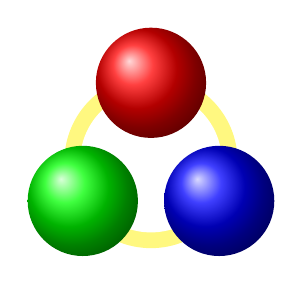
\begin{tikzpicture}
\path[fill=yellow!50!white] (0,0) circle (11mm);
\path[fill=white] (0,0) circle (9mm);
\foreach \w/\c in {90/red,210/green,330/blue}
{\path[shading=ball,ball color=\c] (\w:1cm) circle (7mm);}
\end{tikzpicture}
\end{tcblisting}

\begin{itemize}

\item 下面是一个列表测试项

\begin{tcblisting}{
  mycode/betweenline={test.hs},
  mycode/betweenline/syntax={haskell},
  mycode/betweenline/highlightlines={1-4},
  listing only,
}
module Main where

import Lib
import 脎\codeHL{Control}吡Control.Lens 

main :: IO ()
main = someFunc 

lst = [x| x <- ['a'..'z']] 
\end{tcblisting}

\end{itemize}

左侧的 \LaTeX 语言高亮似乎有些问题,这个应该是 Pygments 的锅\rlap。

\begin{tcblisting}{
  mycode/betweenline={test.rkt},
  mycode/betweenline/syntax={racket},
  mycode/betweenline/highlightlines={1-6},
  listing only,
}
;; 过程合约 :  in-S? : Natural   → Bool
;; 过程用途 : (in-S?     n   )   = #t 仅当 n 属于 S , 否则为 #f
;; 实参语法 :          Natural ::=  0 | (succ Natural)
(define in-S? 
  (lambda (n)
    (if (zero? n) #t
        (if (>= (- n 3) 0) (in-S? (- n 3))
            #f))))
\end{tcblisting}

泥濠!我是沉积岩!下面是一段一段测试文字:%
\tcblst[haskell]{lst = [x| x <- }
\tcblst[haskell]{['a'..'g']] -- by 沉积岩}\ 
\tcblst{tcolorbox}

\begin{tcblisting}{
  mycode/betweenline={test.lean},
  mycode/betweenline/syntax={lean4},
  mycode/betweenline/highlightlines={1-4},
  listing only,
}
theorem funext {f₁ f₂ : ∀ (x : α), β x} (h : ∀ x, f₁ x = f₂ x) : f₁ = f₂ := by
  show extfunApp (Quotient.mk' f₁) = extfunApp (Quotient.mk' f₂)
  apply congrArg
  apply Quotient.sound
  exact h
\end{tcblisting}

\end{multicols*}

\newpage
\begin{multicols*}{2}
\section{\tcblst{tcolorbox} 代码块测试}

\subsection{\tcblst{tcolorbox} 代码块测试}

\subsubsection{\tcblst{tcolorbox} 代码块测试}

\tcbinputlisting{
  mycode/betweenline={test.tex},
  mycode/betweenline/syntax={latex},
  mycode/betweenline/highlightlines={5-7},
  listing above text,
  listing file=statics/code/test.tex
}

\begin{itemize}

\item 下面是一个列表测试项

\tcbinputlisting{
  mycode/betweenline={test.hs},
  mycode/betweenline/syntax={haskell},
  mycode/betweenline/highlightlines={1-3,6-9},
  listing only,
  listing file=statics/code/test.hs
}

\end{itemize}

左侧的 \LaTeX 语言高亮似乎有些问题,这个应该是 Pygments 的锅\rlap。

\tcbinputlisting{
  mycode/betweenline={test.rkt},
  mycode/betweenline/syntax={racket},
  mycode/betweenline/highlightlines={1-6},
  listing only,
  listing file=statics/code/test.rkt
}

泥濠!我是沉积岩!下面是一段一段测试文字:%
\tcblst[haskell]{lst = [x| x <- }
\tcblst[haskell]{['a'..'g']] -- by 沉积岩}\ 
\tcblst{tcolorbox}

\tcbinputlisting{
  mycode/betweenline={test.lean},
  mycode/betweenline/syntax={lean4},
  mycode/betweenline/highlightlines={1-4},
  listing only,
  listing file=statics/code/test.lean
}

\end{multicols*}

\newpage 
% \input{tests/tikz-01}
% % keyval test
\makeatletter
\define@key{family}{color}[black]{\color{#1}}
\define@key{family}{font}{#1}
\def\mybox{%
  \@ifnextchar[% 如果下一个字符是 [ 
  \@mybox%     % 那么调用带参数的版本
  {\@mybox[]}% % 否则调用不带参数的版本
}
\def\@mybox[#1]#2{%
  \setkeys{family}{#1}%
  #2
  % some operations to typeset #2
}
\makeatother

% \mybox[%
%   color = red,
%   % font  = \ttfamily
% ]{%
%   This is my box%
% }%

\pgfkeys{
  /family/.is family,
  /family,
  color/.initial = black,
  color/.code    = \color{#1},
  font/.initial  = \normalfont,
  font/.code     = #1,
}
\renewcommand\mybox[2][]{%
  \pgfkeys{/family, #1}%
  #2
}

\pgfkeysvalueof{/family/color}

\mybox[%
  color = red,
  % font  = \ttfamily
]{%
  This is my box%
}%

\pgfkeysvalueof{/family/color}

% \def\helloworld{Hello, world!}
% \pgfkeyslet{/my family/my key}{\helloworld}
% \pgfkeysvalueof{/my family/my key}

% \pgfkeyssetvalue{/my family/my key}{Hello, world!}
% \pgfkeysgetvalue{/my family/my key}{\helloworld}
% \helloworld
% \usepgfmodule{oo}

\pgfooclass{stamp}{
  % This is the class stamp

  \method stamp() { % The constructor
  }

  \method apply(#1,#2) { % Causes the stamp to be shown at coordinate (#1,#2)
    % Draw the stamp:
    \node [rotate=20,font=\huge] at (#1,#2) {Passed};
  }
}

\pgfoonew \mystamp=new stamp()

\begin{tikzpicture}
  \mystamp.apply(1,2)
  \mystamp.apply(3,4)
\end{tikzpicture}

\pgfooclass{mathobj}{
  \attribute form LaTeX ;
  \attribute form Verb  ;
  \attribute type       ;
  \method mathobj(#1) {%
    \pgfooset{form LaTeX}{\ensuremath{#1}}%
  }
  \method print LaTeX() {%
    \pgfoovalueof{form LaTeX}%
  }
}

\pgfoonew\mymathobj=new mathobj(x^2)

\mymathobj.print LaTeX()
% \let\ph=\phantom
\let\hph=\hphantom
\let\vph=\vphantom
\let\mrel=\mathrel
\let\mbin=\mathbin
\let\mllap=\mathllap
\let\mrlap=\mathrlap
\let\mclap=\mathclap

\newdimen\mathHLfboxsep
\mathHLfboxsep=0pt                             % 默认值 mathHLfboxrule
\newdimen\mathHLfboxrule
\mathHLfboxrule=0.2pt                          % 默认值 mathHLfboxsep
\newcommand{\mathHL}[2]{{%                     % 高亮
  \setlength{\fboxsep}{\mathHLfboxsep}%        % 边距
  \setlength{\fboxrule}{\mathHLfboxrule}%      % 边框宽度
  \colorbox{#1}{\ensuremath{#2}}%
}}

\def\vts#1{\lvert#1\rvert}                     % 竖线 ||
\def\prs#1{\left(#1\right)}                    % 括号 ()
\def\bcs#1{\left\{#1\right\}}                  % 括号 {}
\def\bks#1{\left[#1\right]}                    % 括号 []
\def\plr{\vph{(fg)}}                           % 柱子, 用于指定盒子的最小高度
\def\etc{\textrm{etc}}                         % 对应省略号
\def\wld{\_}                                   % 通配符

% 值构造器
\def\cons{\mbin{.}}                            % 对应积类型 , 同 ","
\def\ethr{\mbin{\vert}}                        % 对应和类型 , 同 "|"

% 几个类型 : 对象 , 范畴 , 态射 , 函子 , 自然变换
\def\Series#1#2#3{%                            % 大类, 用于加高亮色
  \mathHL{#1! #2}%
  {\plr\smash{#3}}
}
\def\objSeries#1#2{\Series{blue}{#1}{\sf #2}}  % 对象类型 , 蓝色底色 , sf 字体
\def\arrSeries#1#2{\Series{pink}{#1}{#2}}      % 箭头类型 , 红色底色 , 普通字体

\def\obj#1{\objSeries{10}{#1}}                 % 对象
\def\cat#1{\objSeries{30}{#1}}                 % 范畴
\def\arr#1{\arrSeries{90!Orchid}{#1}}          % 箭头
\def\fct#1{\arrSeries{10!Orchid}{#1}}          % 函子 
\def\ntf#1{\arrSeries{40!Orchid}{#1}}          % 自然变换

% 常用变量
\makeatletter
\def\varFreqUse#1#2{
  \expandafter\newcommand\expandafter{\csname #1#2\endcsname}[1][]%
  {\@ifnextchar p%
    {\csname #1#2@A\endcsname{##1}}%
    {\csname #1#2@B\endcsname{##1}}%
  }
  \expandafter\def\csname #1#2@A\endcsname##1p%
  {\@ifnextchar p%
    {\csname #1#2@A@A\endcsname{##1}p}%
    {\csname #1#2@A@B\endcsname{##1}p}%
  }
  \expandafter\def\csname #1#2@A@A\endcsname##1pp%
  {\csname #1\endcsname {#2_{##1}''}}
  \expandafter\def\csname #1#2@A@B\endcsname##1p%
  {\csname #1\endcsname {#2_{##1}'}}
  \expandafter\def\csname #1#2@B\endcsname##1%
  {\csname #1\endcsname {#2_{##1}}}
}
\varFreqUse{obj}{0}                            % 对象 0
\varFreqUse{obj}{1}                            % 对象 1
\varFreqUse{obj}{c}                            % 对象 c
\varFreqUse{obj}{d}                            % 对象 d
\varFreqUse{arr}{f}                            % 箭头 f
\varFreqUse{arr}{g}                            % 箭头 g
\varFreqUse{fct}{F}                            % 函子 F
\varFreqUse{fct}{G}                            % 函子 G
\varFreqUse{cat}{C}                            % 范畴 C
\varFreqUse{cat}{D}                            % 范畴 D
\varFreqUse{cat}{Cat}                          % 范畴 Cat
\varFreqUse{cat}{Set}                          % 范畴 Set
\makeatother
% 打印方法名
\newcommand{\opr}[2][\catC]{                   % 方法的名称
  \plr\smash{\overset{\mclap{\small #1}}{#2}}
}
\def\rst#1undr#2{
  {}^{}_{\smash{:#2}}{\plr\smash{#1}}
}
\newcommand{\id}[1][\obj c]{
  \rst{\textrm{id}}undr#1
}

$\obj a,\obj b,\obj c$ , $\cat C$ \par
$\arr f$ , $\ntf \eta$ , $\fct F$ \par
$\obj0$ , $\obj1$ , $\objc[1]pp$ , $\objd[1]p$ , $\objd[i]p$ \par
$\arrf$ , $\arrf[1]p$ , $\arrg[2]pp$ \par
$\fctF$ , $\fctG$
% % 一系列别名
\let\ph=\phantom
\let\hph=\hphantom
\let\vph=\vphantom
\let\mrel=\mathrel
\let\mbin=\mathbin
\let\mllap=\mathllap
\let\mrlap=\mathrlap
\let\mclap=\mathclap

\def\vts#1{\lvert#1\rvert}                     % 竖线 ||
\def\prs#1{\left(#1\right)}                    % 括号 ()
\def\bcs#1{\left\{#1\right\}}                  % 括号 {}
\def\bks#1{\left[#1\right]}                    % 括号 []
\def\plr{\vph{(fg)}}                           % 柱子, 用于指定盒子的最小高度
\def\etc{\textrm{etc}}                         % 对应省略号
\def\wld{\_}                                   % 通配符

% 用于注册需要被高亮的数学对象
\def\RegistMathHL#1BG#2Font#3{
  \colorlet{color#1}{#2}
  \expandafter\newif\csname ifmathHLcolor#1\endcsname    % 确认是否开启背景高亮
  \expandafter\def\csname #1\endcsname##1{%
    \setlength{\fboxsep}{0pt}%
    \setlength{\fboxrule}{0pt}%
    \let\intermediate=\relax
    \csname ifmathHLcolor#1\endcsname{%
      \gdef\intermediate{\colorbox{color#1}}%
    }\else{%
      \gdef\intermediate{\fbox}%
    }\fi%
    \intermediate{\ensuremath{\plr\smash{#3 ##1}}}%
  }
  \csname mathHLcolor#1true\endcsname                    % 默认开启背景高亮
}

% 注册几种类型 : 对象 , 范畴 , 态射 , 函子 , 自然变换
\RegistMathHL{obj}BG{blue!10}Font{\sf}
\RegistMathHL{cat}BG{blue!30}Font{\sf}
\RegistMathHL{arr}BG{pink!90!Orchid}Font{}
\RegistMathHL{fct}BG{pink!10!Orchid}Font{}
\RegistMathHL{ntf}BG{pink!40!Orchid}Font{}

% 测试
$\obj a,\obj b,\obj c$ , $\cat C$ \par
$\arr f$ , $\ntf \eta$ , $\fct F$ \par

% 常用变量
\makeatletter
\def\RegistVarFreq#1#2{
  \expandafter\newcommand\expandafter{\csname #1#2\endcsname}[1][]%
  {\@ifnextchar p%
    {\csname #1#2@A\endcsname{##1}}%
    {\csname #1#2@B\endcsname{##1}}%
  }
  \expandafter\def\csname #1#2@A\endcsname##1p%
  {\@ifnextchar p%
    {\csname #1#2@A@A\endcsname{##1}p}%
    {\csname #1#2@A@B\endcsname{##1}p}%
  }
  \expandafter\def\csname #1#2@A@A\endcsname##1pp%
  {\csname #1\endcsname {#2_{##1}''}}
  \expandafter\def\csname #1#2@A@B\endcsname##1p%
  {\csname #1\endcsname {#2_{##1}'}}
  \expandafter\def\csname #1#2@B\endcsname##1%
  {\csname #1\endcsname {#2_{##1}}}
}
\makeatother

% 注册几个常用变量
\RegistVarFreq{obj}{0}                            % 对象 0
\RegistVarFreq{obj}{1}                            % 对象 1
\RegistVarFreq{obj}{c}                            % 对象 c
\RegistVarFreq{obj}{d}                            % 对象 d
\RegistVarFreq{arr}{f}                            % 箭头 f
\RegistVarFreq{arr}{g}                            % 箭头 g
\RegistVarFreq{fct}{F}                            % 函子 F
\RegistVarFreq{fct}{G}                            % 函子 G
\RegistVarFreq{cat}{C}                            % 范畴 C
\RegistVarFreq{cat}{D}                            % 范畴 D
\RegistVarFreq{cat}{Cat}                          % 范畴 Cat
\RegistVarFreq{cat}{Set}                          % 范畴 Set

% 测试
$\obj0$ , $\obj1$ , $\objc[1]pp$ , $\objd[1]p$ , $\objd[i]p$ \par
$\arrf$ , $\arrf[1]p$ , $\arrg[2]pp$ \par
$\fctF$ , $\fctG$

% 打印方法名
% \def\RegistMathOpr#1{%
%   \expandafter\def\csname #1\endcsname{%
%     \@ifnextchar [%
%       {\csname #1@A\endcsname}%
%       {\csname #1@B\endcsname}%
%   }%
%   \expandafter\def\csname #1@A\endcsname[##1]##2{%
%     Mandatory ##2 , Optional ##1%
%   }%
%   \expandafter\def\csname #1@B\endcsname##1{%
%     \csname #1@A\endcsname[Default]{##1}
%   }%
% }



\newcommand{\opr}[2][\catC]{                      % 方法的名称
  \plr\smash{\overset{\mclap{\small #1}}{#2}}
}

\makeatletter
\def\testOpt#1{
  \@ifnextchar <%
  {\testOpt@A#1}%
  {\testOpt@B#1}%
}
\def\testOpt@A#1<#2>{%
  Mandatory {\ttfamily #2} , Optional {\ttfamily #1}%
}%
\def\testOpt@B#1{%
  \testOpt@A#1[d]
}%
\makeatother

\testOpt{A}<x>
% \testOpt@A x

\makeatletter
\def\RegistMathOpr#1#2{
  \expandafter\def\csname #1\endcsname{%
    \@ifnextchar <%
      {\csname #1@A\endcsname}%
      {\csname #1@B\endcsname}%
  }%
  \expandafter\def\csname #1@A\endcsname<##1>{%
    \plr\smash{\overset{\mclap{\small ##1}}{#2}}
  }%
  \expandafter\def\csname #1@B\endcsname{%
    \csname #1@A\endcsname<\catC>
  }%
}
\makeatother

\RegistMathOpr{cattimes}{\times}

$\cattimes<\catD>$\par
$\cattimes$
% % 一系列别名
\let\ph=\phantom
\let\hph=\hphantom
\let\vph=\vphantom
\let\mrel=\mathrel
\let\mbin=\mathbin
\let\mllap=\mathllap
\let\mrlap=\mathrlap
\let\mclap=\mathclap

\def\vts#1{\lvert#1\rvert}                     % 竖线 ||
\def\prs#1{\left(#1\right)}                    % 括号 ()
\def\bcs#1{\left\{#1\right\}}                  % 括号 {}
\def\bks#1{\left[#1\right]}                    % 括号 []
\def\plr{\vph{(fg)}}                           % 柱子, 用于指定盒子的最小高度
\def\etc{\textrm{etc}}                         % 对应省略号
\def\wld{\_}                                   % 通配符

\makeatletter
\def\opr{%
  \@ifnextchar<
  {\opr@Q}
  {f}%
}
\def\opr@Q<{%
  \@ifnextchar<%
  {\opr@YopY}
  {\opr@YopX}%
}
\def\opr@YopX#1{%
  \@ifnextchar<%
  {\opr@YopX@YopY{#1}}
  {\opr@YopX@NopY{#1}}%
}
\def\opr@YopX@YopY#1<#2{%
  (#2~#1~f)
}
\def\opr@YopX@NopY#1{%
  (#1~f)
}
\def\opr@YopY<#1{%
  \@ifnextchar<%
  {\opr@YopY@YopX{#1}}
  {\opr@YopY@NopX{#1}}%
}
\def\opr@YopY@YopX#1<#2{%
  (#1~#2~f)%
  %=#2~(#1~\_~f)%
}
\def\opr@YopY@NopX#1{%
  (#1~\_~f)%
}

\def\RegistOprBin#1#2{
  \expandafter\def\csname #1\endcsname{%
    \@ifnextchar<
    {\csname #1@\endcsname}
    {#2}%
  }
  \expandafter\def\csname #1@\endcsname<{%
    \@ifnextchar<%
    {\csname #1@YopY@\endcsname}
    {\csname #1@YopX@\endcsname}%
  }
  \expandafter\def\csname #1@YopX@\endcsname##1{%
    \@ifnextchar<%
    {\csname #1@YopX@YopY\endcsname{##1}}
    {\csname #1@YopX@NopY\endcsname{##1}}%
  }
  \expandafter\def\csname #1@YopX@NopY\endcsname##1{%
    (##1~#2)%
  }
  \expandafter\def\csname #1@YopX@YopY\endcsname##1<##2{%
    (##2~##1~#2)%
  }
  \expandafter\def\csname #1@YopY@\endcsname<##1{%
    \@ifnextchar<%
    {\csname #1@YopY@YopX\endcsname{##1}}
    {\csname #1@YopY@NopX\endcsname{##1}}%
  }
  \expandafter\def\csname #1@YopY@NopX\endcsname##1{%
    (##1~\_~#2)% 
  }
  \expandafter\def\csname #1@YopY@YopX\endcsname##1<##2{%
    (##1~##2~#2)%
  }
}
\makeatother

\RegistOprBin{test}{g}% typeZ <- typeX <- type Y

\begin{tblr}{
  colspec={Q[l]Q[r]},
  hlines,vlines,
  rows = {LightGray}
}
\tcblst{$\test=z_u$} &
$\test=z_u$ 
\\
\tcblst{$\test<{x_u}=z_u$} &
$\test<{x_u}=z_u$ 
\\
\tcblst{$\test<{x_u}<{y_u}=z_u$} &
$\test<{x_u}<{y_u}=z_u$ 
\\
\tcblst{$\test<<{y_u}=z_u$} &
$\test<<{y_u}=z_u$ 
\\
\tcblst{$\test<<{y_u}<{x_u}=z_u$} &
$\test<<{y_u}<{x_u}=z_u$ 
\\
\end{tblr} % currying operator
% \newline

\let\xpndaft=\expandafter
\makeatletter
\def\RegistMathObjField#1.#2={%
  \@ifnextchar[%
    {\RegistMathObjFieldAvecArgs#1.#2=}%
    {\RegistMathObjFieldSansArgs#1.#2=}%
}
\def\RegistMathObjFieldAvecArgs#1.#2=[#3]#4{%
  \xpndaft\newcommand\xpndaft{\csname #1.#2\endcsname}[#3]{#4}%
}
\def\RegistMathObjFieldSansArgs#1.#2=#3{%
  \xpndaft\newcommand\xpndaft{\csname #1.#2\endcsname}{#3}%
}
\makeatother
\def\RegistMathObj#1=#2:#3{
  \def\this{\RegistMathObjField{#1}}
  \xpndaft\newcommand\xpndaft{\csname #1\endcsname}{#1}
  \this.{get_eqn}={#2}
  \this.{get_typ}={#3}
  \this.{set_eqn}=[1]{%
    \xpndaft\renewcommand\xpndaft{\csname #1.get_eqn\endcsname}[1]{##1}
  }
  \this.{set_typ}=[1]{%
    \xpndaft\renewcommand\xpndaft{\csname #1.get_typ\endcsname}[1]{##1}
  }
}

\def\print #1{%
  \csname #1.get_eqn\endcsname%
}
\def\check #1{%
  \csname #1.get_eqn\endcsname :
  \print{\csname #1.get_typ\endcsname}%
}

\RegistMathObj{catCat}={{\sf Cat}}:{???}
\RegistMathObj{catC}={{\sf C}}:{\catCat}
\RegistMathObj{objc}={{\sf c}}:{\catC}

\begin{tblr}{
  colspec={Q[l]Q[l]},
  hlines,vlines,
  rows = {LightGray}
}
\tcblst{$\print{\objc}$} & $\print{\objc}$ \\
\tcblst{$\print{\catC}$} & $\print{\catC}$ 
\end{tblr}

\begin{tblr}{
  colspec={Q[l]Q[l]},
  hlines,vlines,
  rows = {LightGray}
}
\tcblst{$\check{\objc}$} & $\check{\objc}$ \\
\tcblst{$\check{\catC}$} & $\check{\catC}$ 
\end{tblr}
 % types
% \input{tests/math-05} % union types , match
% \let\xpndaft=\expandafter
\let\ncm=\newcommand
\let\rcm=\renewcommand
% ----- 排版相关
\newcommand{\cfbox}[2][blue]{%
  \setlength{\fboxsep}{0pt}%
  \setlength{\fboxrule}{0.4pt}%
  \colorlet{currentcolor}{.}%
  {\color{#1}%
  \fbox{\color{currentcolor}\ensuremath{#2}}}%
}
\let\ph=\phantom
\let\hph=\hphantom
\let\vph=\vphantom
\let\mrel=\mathrel
\let\mbin=\mathbin
\let\mop=\mathop
\let\mllap=\mathllap                 % 根据文本右侧对齐
\let\mrlap=\mathrlap                 % 根据文本左侧对齐
\let\mclap=\mathclap                 % 根据文本中央对齐
\def\vts#1{\lvert#1\rvert}
\def\prs#1{\left(#1\right)}
\def\bcs#1{\left\{#1\right\}}
\def\bks#1{\left[#1\right]}
\def\plr#1{\vph{(fg)}\smash{#1}}     % 柱子
\def\etc{\plr{\rm etc}}              % 省略号
\def\occ{\plr{\tt\_}}                % 占位符
% ----- 变量注册模板 带高亮
\def\RegistVarType#1BG#2Font#3{
  \colorlet{color#1}{#2}
  \xpndaft\newif\csname ifColorVarType#1\endcsname    % 确认是否开启背景高亮
  \xpndaft\def\csname #1\endcsname##1{{%
    \setlength{\fboxsep}{0pt}%
    \setlength{\fboxrule}{0pt}%
    \let\intermediate=\relax
    \csname ifColorVarType#1\endcsname{%
      \gdef\intermediate{\colorbox{color#1}}%
    }\else{%
      \gdef\intermediate{\fbox}%
    }\fi%
    \intermediate{\ensuremath{\plr{#3 ##1}}}%
  }}
  \csname ColorVarType#1true\endcsname                    % 默认开启背景高亮
}
% ----- 二元操作符注册模板
\makeatletter
\def\RegistOprBin#1Form#2Eval#3OccA#4OccB#5EvU#6EvU#7EvU#8{%
  \xpndaft\def\csname #1\endcsname{%
    \@ifnextchar [
    {\csname #1@optionGet\endcsname}
    {\def\cache{#2}
     \csname #1@relax\endcsname
    }
  }
  \xpndaft\def\csname #1@optionGet\endcsname[##1]{
    \def\cache{#2[##1]}
    \csname #1@relax\endcsname
  }
  \xpndaft\def\csname #1@relax\endcsname{%
    \@ifnextchar<
    {\csname #1@\endcsname}
    {\cache}%
  }
  \xpndaft\def\csname #1@\endcsname<{%
    \@ifnextchar<
    {\csname #1@YopY@\endcsname}
    {\csname #1@YopX@\endcsname}%
  }
  \xpndaft\def\csname #1@YopX@\endcsname##1{%
    \@ifnextchar p%
      {\csname #1@YopX@Yp@\endcsname{##1}}%
      {\csname #1@YopX@Np@\endcsname{##1}}%
  }
  \xpndaft\def\csname #1@YopX@Np@\endcsname##1{%
    \@ifnextchar<
    {\csname #1@YopX@Np@YopY@\endcsname{##1}}%
    {\csname #1@YopX@Np@NopY\endcsname{##1}}%
  }
  \xpndaft\def\csname #1@YopX@Np@NopY\endcsname##1{\cfbox{#3{\cache}{##1}{#5}}}
  \xpndaft\def\csname #1@YopX@Np@YopY@\endcsname##1<##2{%
    \@ifnextchar p
    {\csname #1@YopX@Np@YopY@Yp\endcsname{##1}{##2}}% 
    {\csname #1@YopX@Np@YopY@Np\endcsname{##1}{##2}}%
  }
  \xpndaft\def\csname #1@YopX@Np@YopY@Np\endcsname##1##2{\cfbox{#6{\cfbox{#3{\cache}{##1}{}}}{##2}}}
  \xpndaft\def\csname #1@YopX@Np@YopY@Yp\endcsname##1##2p{\cfbox{\prs{#6{\cfbox{#3{\cache}{##1}{}}}{##2}}}}
  \xpndaft\def\csname #1@YopX@Yp@\endcsname##1p{%
    \@ifnextchar<
    {\csname #1@YopX@Yp@YopY@\endcsname{##1}}%
    {\csname #1@YopX@Yp@NopY\endcsname{##1}}%
  }
  \xpndaft\def\csname #1@YopX@Yp@NopY\endcsname##1{\cfbox{\prs{#3{\cache}{##1}{#5}}}}
  \xpndaft\def\csname #1@YopX@Yp@YopY@\endcsname##1<##2{%
    \@ifnextchar p
    {\csname #1@YopX@Yp@YopY@Yp\endcsname{##1}{##2}}%
    {\csname #1@YopX@Yp@YopY@Np\endcsname{##1}{##2}}%
  }
  \xpndaft\def\csname #1@YopX@Yp@YopY@Np\endcsname##1##2{\cfbox{#7{\cfbox{\prs{#3{\cache}{##1}{#5}}}}{##2}}}
  \xpndaft\def\csname #1@YopX@Yp@YopY@Yp\endcsname##1##2p{\cfbox{\prs{#7{\cfbox{\prs{#3{\cache}{##1}{#5}}}}{##2}}}}

  \xpndaft\def\csname #1@YopY@\endcsname<##1{%
    \@ifnextchar p%
    {\csname #1@YopY@Yp@\endcsname{##1}}%
    {\csname #1@YopY@Np@\endcsname{##1}}%
  }
  \xpndaft\def\csname #1@YopY@Np@\endcsname##1{%
    \@ifnextchar<
    {\csname #1@YopY@Np@YopX@\endcsname{##1}}%
    {\csname #1@YopY@Np@NopX\endcsname{##1}}%
  }
  \xpndaft\def\csname #1@YopY@Np@NopX\endcsname##1{\cfbox{#3{\cache}\occ{##1}}}
  \xpndaft\def\csname #1@YopY@Np@YopX@\endcsname##1<##2{%
    \@ifnextchar p
    {\csname #1@YopY@Np@YopX@Yp\endcsname{##1}{##2}}%
    {\csname #1@YopY@Np@YopX@Np\endcsname{##1}{##2}}%
  }
  \xpndaft\def\csname #1@YopY@Np@YopX@Np\endcsname##1##2{\cfbox{#8{\cfbox{#3{\cache}{}{##1}}}{##2}}??}
  \xpndaft\def\csname #1@YopY@Np@YopX@Yp\endcsname##1##2p{\cfbox{\prs{#6{\cfbox{#3{\cache}{##2}{}}}{##1}}}??}
  \xpndaft\def\csname #1@YopY@Yp@\endcsname##1p{%
    \@ifnextchar<
    {\csname #1@YopY@Yp@YopX@\endcsname{##1}}%
    {\csname #1@YopY@Yp@NopX\endcsname{##1}}%
  }
  \xpndaft\def\csname #1@YopY@Yp@NopX\endcsname##1{\prs{#3{\cache}\occ{##1}}}
  \xpndaft\def\csname #1@YopY@Yp@YopX@\endcsname##1<##2{%
    \@ifnextchar p
    {\csname #1@YopY@Yp@YopX@Yp\endcsname{##1}{##2}}%
    {\csname #1@YopY@Yp@YopX@Np\endcsname{##1}{##2}}%
  }
  \xpndaft\def\csname #1@YopY@Yp@YopX@Np\endcsname##1##2{##2\prs{#3{\cache}\occ{##1}}}
  \xpndaft\def\csname #1@YopY@Yp@YopX@Yp\endcsname##1##2p{\prs{##2\prs{#3{\cache}\occ{##1}}}}
}
\makeatother
% ----- 二元操作符求值模板
\ncm{\OprBinEvlPo}[3]{\plr{{#3}{#2}\mop{#1}}}                  % 二元 后缀形式
\ncm{\OprBinEvlPoR}[3]{
  \let\OprBinEvlPoRtempA=#3
  \let\OprBinEvlPoRtempB=#2
  \plr{{#3}{#2}\mop{#1}}
}                  % 二元 后缀形式
\ncm{\OprBinEvlIn}[3]{\plr{{#2}\mbin{#1}{#3}}}                 % 二元 中缀形式
\ncm{\OprBinEvlInS}[3]{\plr{{}_{\plr{{#2}\mbin{#1}{}}}{#3}}}   % 二元 中缀形式
\ncm{\OprUniEvlPo}[2]{\plr{{#2}\mop{#1}}}                      % 一元 后缀形式
\ncm{\OprUniEvlPoS}[2]{\plr{{}_{\plr{#2}}\mop{#1}}}            % 一元 后缀形式
\ncm{\OprUniEvlPr}[2]{\plr{\mop{#1}{#2}}}                      % 一元 前缀形式
% ----- 二元操作符形式模板(不包括 Hom 函子)
\def\RegistOprBinFormA#1Disp#2Dflt#3{
  \xpndaft\ncm\xpndaft{\csname#1\endcsname}[1][#3]{\plr{
    \overset{\mclap{\small\plr{}}}{
    \underset{\mclap{\small\plr{##1}}}
    {\plr{#2}}}
  }}
}
\def\RegistOprBinFormB#1Dflt#2{
  \xpndaft\ncm\xpndaft{\csname#1\endcsname}[1][#2]{\plr{
    \xrightarrow[{\small\plr{##1}}]{}   
  }}
}

% ----- 注册变量
\RegistVarType{obj}BG{pink}Font{\sf}
\RegistVarType{cat}BG{Rhodamine}Font{\sf}
\RegistVarType{arr}BG{SpringGreen}Font{}
\RegistVarType{fct}BG{YellowGreen}Font{}
\RegistVarType{ntf}BG{LightBlue}Font{}
% ----- 注册二元运算形式
\RegistOprBinFormA{catAddForm}Disp{+}Dflt{\cat C}
\RegistOprBinFormA{catMulForm}Disp{\times}Dflt{\cat C}
\RegistOprBinFormB{catHomForm}Dflt{\cat C}
% ----- 注册二元运算
\RegistOprBin{test}Form{{\rm Opr}}Eval{\OprBinEvlPo}OccA{\occ}OccB{}EvU{\OprUniEvlPo}EvU{\OprUniEvlPo}EvU{\OprUniEvlPo}
\RegistOprBin{catAdd}Form{\catAddForm}Eval{\OprBinEvlIn}OccA{\occ}OccB{\occ}EvU{\OprUniEvlPr}EvU{\OprUniEvlPo}EvU{\OprUniEvlPo}
\RegistOprBin{catMul}Form{\catMulForm}Eval{\OprBinEvlIn}OccA{\occ}OccB{\occ}EvU{\OprUniEvlPr}EvU{\OprUniEvlPo}EvU{\OprUniEvlPo}
\RegistOprBin{catHom}Form{\catHomForm}Eval{\OprBinEvlIn}OccA{\occ}OccB{\occ}EvU{\OprUniEvlPr}EvU{\OprUniEvlPo}EvU{\OprUniEvlPo}
\RegistOprBin{catExp}Form{\catHomForm}Eval{\OprBinEvlInS}OccA{\occ}OccB{\occ}EvU{\OprUniEvlPr}EvU{\OprUniEvlPo}EvU{\OprUniEvlPoS}


\begin{tblr}{
  colspec={Q[l]Q[r]},
  hlines,vlines,
  rows = {LightGray}
}
\tcblst{$\test$} &
$\test$ 
\\
\tcblst{$\test<{x_u}$} &
$\test<{x_u}$ 
\\
\tcblst{$\test<{x_u}<{y_u}$} &
$\test<{x_u}<{y_u}$ 
\\
\tcblst{$\test<{x_u}<{y_u}p$} &
$\test<{x_u}<{y_u}p$ 
\\
\tcblst{$\test<{x_u}p$} &
$\test<{x_u}p$
\\
\tcblst{$\test<{x_u}p<{y_u}$} &
$\test<{x_u}p<{y_u}$
\\
\tcblst{$\test<{x_u}p<{y_u}p$} &
$\test<{x_u}p<{y_u}p$
\\
\tcblst{$\test<<{y_u}$} &
$\test<<{y_u}$ 
\\
\tcblst{$\test<<{y_u}<{x_u}$} &
$\test<<{y_u}<{x_u}$ 
\\
\tcblst{$\test<<{y_u}<{x_u}p$} &
$\test<<{y_u}<{x_u}p$ 
\\
\tcblst{$\test<<{y_u}p$} &
$\test<<{y_u}p$ 
\\
\tcblst{$\test<<{y_u}p<{x_u}$} &
$\test<<{y_u}p<{x_u}$ 
\\
\tcblst{$\test<<{y_u}p<{x_u}p$} &
$\test<<{y_u}p<{x_u}p$ 
\\
\end{tblr}
\begin{tblr}{
  colspec={Q[l]Q[r]},
  hlines,vlines,
  rows = {LightGray}
}
\tcblst{$\catExp[\cat D]$} &
$\catExp[\cat D]$ 
\\
\tcblst{$\catExp[\cat D]<{x_u}$} &
$\catExp[\cat D]<{x_u}$ 
\\
\tcblst{$\catExp[\cat D]<{x_u}<{y_u}$} &
$\catExp[\cat D]<{x_u}<{y_u}$ 
\\
\tcblst{$\catExp[\cat D]<{x_u}<{y_u}p$} &
$\catExp[\cat D]<{x_u}<{y_u}p$ 
\\
\tcblst{$\catExp[\cat D]<{x_u}p$} &
$\catExp[\cat D]<{x_u}p$
\\
\tcblst{$\catExp[\cat D]<{x_u}p<{y_u}$} &
$\catExp[\cat D]<{x_u}p<{y_u}$
\\
\tcblst{$\catExp[\cat D]<{x_u}p<{y_u}p$} &
$\catExp[\cat D]<{x_u}p<{y_u}p$
\\
\tcblst{$\catExp[\cat D]<<{y_u}$} &
$\catExp[\cat D]<<{y_u}$ 
\\
\tcblst{$\catExp[\cat D]<<{y_u}<{x_u}$} &
$\catExp[\cat D]<<{y_u}<{x_u}$ 
\\
\tcblst{$\catExp[\cat D]<<{y_u}<{x_u}p$} &
$\catExp[\cat D]<<{y_u}<{x_u}p$ 
\\
\tcblst{$\catExp[\cat D]<<{y_u}p$} &
$\catExp[\cat D]<<{y_u}p$ 
\\
\tcblst{$\catExp[\cat D]<<{y_u}p<{x_u}$} &
$\catExp[\cat D]<<{y_u}p<{x_u}$ 
\\
\tcblst{$\catExp[\cat D]<<{y_u}p<{x_u}p$} &
$\catExp[\cat D]<<{y_u}p<{x_u}p$ 
\\
\end{tblr}

% 测试
{\ColorVarTypeobjfalse
$\obj a$ , $\obj b$
}, 
$\obj c$ , $\obj d$ , 
$\cat C$ \par
$\arr f$ , $\fct F$ , $\ntf \eta$\par

% $\Add[\cat{Cat}]<{\obj a}<{\obj b}$
% % ----- 注册变量类型
\RegistVarType{obj}BG{pink}Font{\sf}
\RegistVarType{cat}BG{Rhodamine}Font{\sf}
\RegistVarType{arr}BG{SpringGreen}Font{}
\RegistVarType{fct}BG{YellowGreen}Font{}
\RegistVarType{ntf}BG{LightBlue}Font{}
% ----- 注册常用变量
\RegistVarFreqType{obj}Name{c}ppppp
\RegistVarFreqType{obj}Name{init}Disp{0}ppppp
\RegistVarFreqType{obj}Name{term}Disp{1}ppppp
\RegistVarFreqType{arr}Name{f}ppppp
\RegistVarFreqType{cat}Name{C}ppppp
\RegistVarFreqType{cat}Name{D}ppppp
\RegistVarFreqType{cat}Name{I}ppppp
\RegistVarFreqType{fct}Name{F}ppppp
\RegistVarFreqType{fct}Name{G}ppppp
\RegistVarFreqType{ntf}Name{eta}Disp{\eta}ppppp
% ----- 注册常量
\RegistVarFreqType{cat}Name{Cat}Disp{Cat}
\RegistVarFreqType{cat}Name{Set}Disp{Set}
\RegistVarFreqType{cat}Name{Uni}Disp{\text{\ding{192}}}
\RegistVarFreqType{cat}Name{Bin}Disp{\text{\ding{193}}}
\RegistVarFreqType{cat}Name{Tri}Disp{\text{\ding{194}}}
% ----- 注册常量(运算符)
\RegistOprFormTypeAName{objget}Disp{{\rm Obj}}Dflt{\catCat}
\RegistOprFormTypeAName{arrget}Disp{{\rm Arr}}Dflt{\catCat}
\RegistOprFormTypeBName{Homo}Dflt{\catC}                                % hom函子
\RegistOprFormTypeBName{Expo}Dflt{\catC}                                %  ^ 函子
\RegistOprFormTypeAName{Mult}Disp{\times}Dflt{\catC}                    %  × 函子
\RegistOprFormTypeAName{Addt}Disp{+}Dflt{\catC}                         %  + 函子
\RegistOprFormTypeAName{Diag}Disp{{\rm Di}}Dflt{\catC,\catI}            % 对角函子
\RegistOprFormTypeAName{srcget}Disp{{\rm src}}Dflt{\catC}               % 箭头源头
\RegistOprFormTypeAName{target}Disp{{\rm tar}}Dflt{\catC}               % 箭头目标
\RegistOprFormTypeDName{iden}Disp{{\rm id}}Dflt{\objc}                  % 恒等箭头
\RegistOprFormTypeDName{bang}Disp{\text{!}}Dflt{\objc}                  % bang箭头
\RegistOprFormTypeDName{absd}Disp{\text{\textexclamdown}}Dflt{\objc}    % absurd箭头
\RegistOprFormTypeAName{Yone}Disp{\text{よ}}Dflt{\catC}                 % 米田嵌入
\RegistOprFormTypeAName{Yoda}Disp{\text{\small 尤}}Dflt{\catC}          % 尤达嵌入
% ----- 注册求值方式
\RegistOprEvalTypeU{}Form{objget}
\RegistOprEvalTypeU{}Form{arrget}
\RegistOprEvalTypeU{}Form{srcget}
\RegistOprEvalTypeU{}Form{target}
\RegistOprEvalTypeU{}Form{Yone}
\RegistOprEvalTypeU{}Form{Yoda}
\RegistOprEvalTypeB{in}Form{Homo}
\RegistOprEvalTypeB{inx}Form{Expo}
\RegistOprEvalTypeB{in}Form{Mult}
\RegistOprEvalTypeB{in}Form{Addt}
\RegistOprEvalTypeB{in}Form{Diag}
\RegistOprEvalTypeU{n}Form{ntfeta}
% 
\begin{multicols*}{2}

$\objc$ , $\objcpp$ , $\objcppp$ , $\objcppppp$ , $\objcppn1$ , $\objcpn2$ , $\objinit$ , $\objterm$\\
$\arrf$ , $\arrfp$ , $\arrfn1$ , $\arrfpn2$ , \\
$\ntfeta$ , $\ntfetap$ , $\ntfetan1$ , $\ntfetapn1$ , \\
$\catC$ , $\catCp$ , $\catCn1$ , $\catCppn2$ , $\catUni$ , $\catBin$ , $\catTri$\\
$\fctF$ , $\fctFn1$\ , $\fctG$ , $\fctGpn2$ \\
$\Yone$ , $\Yoda$

$\Addt[\catD]$ , 
$\Mult[\catD]$ , 
$\Homo$ , 
$\objget[\catD]$ , 
$\arrget[\catD]$ , 
$\Diag$ ,
$\Diag[\catD,\catUni]$ , 
$\srcget$ , $\target$ ,
$\bang$ , $\bang[\objcpp]$ , $\absd$ , $\iden[\objcpn1]$

\vspace{10pt}

$\evobjget$ , $\evobjget.{\catD}$ , $\evobjget[\catCat].{\catD}p$ \\
$\evobjget$ , $\evarrget.{\catD}$ , $\evarrget[\catCat].{\catD}p$ \\
$\evntfeta$ , $\evntfeta.\objc$ , $\evntfeta.\objc p$

\vspace{10pt}

$\evBpo\arrf{\objcn1}{\objcn2}$    , $\evBpop\arrf{\objcn1}{\objcn2}$    \\
$\evBpoA\arrf{\objcn1}$            ,                                     \\
$\evBpoAp\arrf{\objcn1}$           ,                                     \\
$\evBpoBp\arrf{\objcn2}$           ,                                     \\
$\evBpoAB\arrf{\objcn1}{\objcn2}$  , $\evBpoABp\arrf{\objcn1}{\objcn2}$  \\
$\evBpoApB\arrf{\objcn1}{\objcn2}$ , $\evBpoApBp\arrf{\objcn1}{\objcn2}$ \\
$\evBpoBpA\arrf{\objcn2}{\objcn1}$ , $\evBpoBpAp\arrf{\objcn1}{\objcn2}$

$\evHomo[{\evHomo[\catCat]<{\catC}.{\catD}}]<{\fctF}.{\fctG}$

\vfill\null\columnbreak

$\evHomo$ , \\
$\evHomo.{\objcn1}.{\objcn2}$ , $\evHomo.{\objcn1}.{\objcn2}p$   \\
$\evHomo<{\objcn1}.{\objcn2}$ , $\evHomo<{\objcn1}.{\objcn2}p$   \\
$\evHomo<{\objcn1}p$ ,                                                  \\
$\evHomo<{\objcn1}p.{\objcn2}$ , $\evHomo<{\objcn1}p.{\objcn2}p$ \\
$\evHomo>{\objcn2}.{\objcn1}$ , $\evHomo>{\objcn2}.{\objcn1}p$   \\
$\evHomo>{\objcn2}p$ ,                                                  \\
$\evHomo>{\objcn2}p.{\objcn1}$ , $\evHomo>{\objcn2}p.{\objcn1}p$ \\

$\evExpo$ , \\
$\evExpo.{\objcn1}.{\objcn2}$ , $\evExpo.{\objcn1}.{\objcn2}p$   \\
$\evExpo<{\objcn1}.{\objcn2}$ , $\evExpo<{\objcn1}.{\objcn2}p$   \\
$\evExpo<{\objcn1}p$ ,                                                  \\
$\evExpo<{\objcn1}p.{\objcn2}$ , $\evExpo<{\objcn1}p.{\objcn2}p$ \\
$\evExpo>{\objcn2}.{\objcn1}$ , $\evExpo>{\objcn2}.{\objcn1}p$   \\
$\evExpo>{\objcn2}p$ ,                                                  \\
$\evExpo>{\objcn2}p.{\objcn1}$ , $\evExpo>{\objcn2}p.{\objcn1}p$ 

\end{multicols*}

\newpage

\begin{tblr}{
  colspec={Q[l]Q[r]},
  hlines,vlines,
  rows = {LightGray}
}
\tcblst{$\evHomo$}                      &
$\evHomo$                                  \\
\tcblst{$\evHomo.{\objcn1}.{\objcn2}$}  &
$\evHomo.{\objcn1}.{\objcn2}$              \\
\tcblst{$\evHomo.{\objcn1}.{\objcn2}p$} &
$\evHomo.{\objcn1}.{\objcn2}p$             \\
\tcblst{$\evHomo<{\objcn1}.{\objcn2}$}  &
$\evHomo<{\objcn1}.{\objcn2}$              \\
\tcblst{$\evHomo<{\objcn1}.{\objcn2}p$} &
$\evHomo<{\objcn1}.{\objcn2}p$             \\
\tcblst{$\evHomo<{\objcn1}p$}           &
$\evHomo<{\objcn1}p$                       \\
\tcblst{$\evHomo<{\objcn1}p.{\objcn2}$} &
$\evHomo<{\objcn1}p.{\objcn2}$             \\
\tcblst{$\evHomo<{\objcn1}p.{\objcn2}p$}&
$\evHomo<{\objcn1}p.{\objcn2}p$            \\
\tcblst{$\evHomo>{\objcn2}.{\objcn1}$} &
$\evHomo>{\objcn2}.{\objcn1}$              \\
\tcblst{$\evHomo>{\objcn2}.{\objcn1}p$}&
$\evHomo>{\objcn2}.{\objcn1}p$             \\
\tcblst{$\evHomo>{\objcn2}p$}          &
$\evHomo>{\objcn2}p$                       \\
\tcblst{$\evHomo>{\objcn2}p.{\objcn1}$}&
$\evHomo>{\objcn2}p.{\objcn1}$             \\
\tcblst{$\evHomo>{\objcn2}p.{\objcn1}p$}&
$\evHomo>{\objcn2}p.{\objcn1}p$            \\
\end{tblr}
% -----
\begin{tblr}{
  colspec={Q[l]Q[r]},
  hlines,vlines,
  rows = {LightGray}
}
\tcblst{$\evExpo$}                             &
$\evExpo$                                  \\
\tcblst{$\evExpo.{\objcn1}.{\objcn2}$}  &
$\evExpo.{\objcn1}.{\objcn2}$              \\
\tcblst{$\evExpo.{\objcn1}.{\objcn2}p$} &
$\evExpo.{\objcn1}.{\objcn2}p$             \\
\tcblst{$\evExpo<{\objcn1}.{\objcn2}$}  &
$\evExpo<{\objcn1}.{\objcn2}$              \\
\tcblst{$\evExpo<{\objcn1}.{\objcn2}p$} &
$\evExpo<{\objcn1}.{\objcn2}p$             \\
\tcblst{$\evExpo<{\objcn1}p$}           &
$\evExpo<{\objcn1}p$                       \\
\tcblst{$\evExpo<{\objcn1}p.{\objcn2}$} &
$\evExpo<{\objcn1}p.{\objcn2}$             \\
\tcblst{$\evExpo<{\objcn1}p.{\objcn2}p$}&
$\evExpo<{\objcn1}p.{\objcn2}p$            \\
\tcblst{$\evExpo>{\objcn2}.{\objcn1}$}  &
$\evExpo>{\objcn2}.{\objcn1}$              \\
\tcblst{$\evExpo>{\objcn2}.{\objcn1}p$} &
$\evExpo>{\objcn2}.{\objcn1}p$             \\
\tcblst{$\evExpo>{\objcn2}p$}           &
$\evExpo>{\objcn2}p$                       \\
\tcblst{$\evExpo>{\objcn2}p.{\objcn1}$} &
$\evExpo>{\objcn2}p.{\objcn1}$             \\
\tcblst{$\evExpo>{\objcn2}p.{\objcn1}p$}&
$\evExpo>{\objcn2}p.{\objcn1}p$            \\
\end{tblr}
% ----- 注册变量类型 未来可以考虑用键值对的方式注册
\RegistVarType{obj}[colorBG=pink,font=\sf]
\RegistVarType{cat}[colorBG=Rhodamine,font=\sf]
\RegistVarType{arr}[colorBG=SpringGreen]
\RegistVarType{fct}[colorBG=YellowGreen]
\RegistVarType{ntf}[colorBG=LightBlue]
% ----- 注册常用变量
\RegistVarFamily{c}Type{obj}ppp
\RegistVarFamily{f}Type{arr}ppp
\RegistVarFamily{C}Type{cat}ppp
\RegistVarFamily{D}Type{cat}ppp
\RegistVarFamily{I}Type{cat}ppp
\RegistVarFamily{F}Type{fct}ppp
\RegistVarFamily{G}Type{fct}ppp
\RegistVarFamily{eta}Type{ntf}Disp{\eta}ppp
% ----- 注册常量
\RegistVarFamily{init}Type{obj}Disp{0}ppp
\RegistVarFamily{term}Type{obj}Disp{1}ppp
\RegistVarFamily{Cat}Type{cat}Disp{Cat}
\RegistVarFamily{Set}Type{cat}Disp{Set}
\RegistVarFamily{Uni}Type{cat}Disp{\text{\ding{192}}}
\RegistVarFamily{Bin}Type{cat}Disp{\text{\ding{193}}}
\RegistVarFamily{Tri}Type{cat}Disp{\text{\ding{194}}}
% ----- 注册常量(运算符)
\RegistOpr{objget}TypeADflt{\catCat}Disp{{\rm Obj}}
\RegistOpr{arrget}TypeADflt{\catCat}Disp{{\rm Arr}}
\RegistOpr{Homo}TypeBDflt{\catC}                                % hom函子
\RegistOpr{Expo}TypeBDflt{\catC}                                %  ^ 函子
\RegistOpr{Mult}TypeADflt{\catC}Disp{\times}                    %  × 函子
\RegistOpr{Addt}TypeADflt{\catC}Disp{+}                         %  + 函子
\RegistOpr{Diag}TypeADflt{\catC,\catI}Disp{{\rm Di}}            % 对角函子
\RegistOpr{srcget}TypeADflt{\catC}Disp{{\rm src}}               % 箭头源头
\RegistOpr{target}TypeADflt{\catC}Disp{{\rm tar}}               % 箭头目标
\RegistOpr{iden}TypeDDflt{\objc}Disp{{\rm id}}                  % 恒等箭头
\RegistOpr{bang}TypeDDflt{\objc}Disp{\text{!}}                  % bang箭头
\RegistOpr{absd}TypeDDflt{\objc}Disp{\text{\textexclamdown}}    % absurd箭头
\RegistOpr{Yone}TypeADflt{\catC}Disp{\text{よ}}                 % 米田嵌入
\RegistOpr{Yoda}TypeADflt{\catC}Disp{\text{\small 尤}}          % 尤达嵌入
% 
\begin{multicols*}{2}

$\objc$ , $\objcpp$ , $\objcppp$ , $\objcppn1$ , $\objcpn2$ , $\objinit$ , $\objterm$\\
$\arrf$ , $\arrfp$ , $\arrfn1$ , $\arrfpn2$ , \\
$\ntfeta$ , $\ntfetap$ , $\ntfetan1$ , $\ntfetapn1$ , \\
$\catC$ , $\catCp$ , $\catCn1$ , $\catCppn2$ , $\catUni$ , $\catBin$ , $\catTri$\\
$\fctF$ , $\fctFn1$\ , $\fctG$ , $\fctGpn2$ \\
$\Yone$ , $\Yoda$ ,
$\Addt[\catD]$ , 
$\Mult[\catD]$ , 
$\Homo$ , 
$\objget[\catD]$ , 
$\arrget[\catD]$ , 
$\Diag$ ,
$\Diag[\catD,\catUni]$ , \\
$\srcget$ , $\target$ ,
$\bang$ , $\bang[\objcpp]$ , $\absd$ , $\iden[\objcpn1]$



\vfill\null\columnbreak

\end{multicols*}
% \ExplSyntaxOn

\NewDocumentCommand{\RegisterVarType}{mO{}}{
  \keys_set:nn { ych/type } { color=,font=,#2 }
  \ych_register_type:n {#1}
}

\keys_define:nn { ych/type }{
  color .str_set:N = \l__ych_register_type_color_str,
  font  .str_set:N = \l__ych_register_type_font_str,
}

\cs_new_protected:Nn \ych_register_type:n
{
  \tl_set:Ne \l__ych_register_tmp_tl{
    \str_if_empty:NTF \l__ych_register_type_color_str
    { ##1 }                                                         % without  color
    { \exp_not:N \mathcolor{\l__ych_register_type_color_str}{##1} } % with     color
  }
  \str_if_empty:NF \l__ych_register_type_font_str{
    \tl_set:Ne \l__ych_register_tmp_tl
    { \exp_not:c { math\l__ych_register_type_font_str } { \exp_not:V \l__ych_register_tmp_tl } }
  }
  \exp_args:NNV \cs_set_protected:Nn \__ych_register_tmp:n \l__ych_register_tmp_tl
  \cs_set_eq:cN {#1} \__ych_register_tmp:n
}
\NewDocumentCommand{\RegisterVarFreqType}{O{5}mm}{
  % #1 = allowed numbers of primes
  % #2 = type previously defined
  % #3 = tokens to incorporate in the abbreviation
  \bool_lazy_and:nnTF { \tl_if_single_p:n {#3} } { \token_if_cs_p:N #3 }{
    \ych_register_freq:nnne {#1} {#2} {#3} { \cs_to_str:N #3 }
  }
  {
    \ych_register_freq:nnnn {#1} {#2} {#3} {#3}
  }
}

\cs_new_protected:Nn \ych_register_freq:nnnn{
  \int_step_inline:nnn {0} {#1}{
    \cs_new_protected:cpe { #2#4 \prg_replicate:nn {##1} {p} }{
      \exp_not:c {#2} {#3} \prg_replicate:nn {##1} {\exp_not:N '}
    }
    \cs_new_protected:cpe { #2#4 \prg_replicate:nn {##1} {p} n } ####1{
      \exp_not:c {#2} {#3} \prg_replicate:nn {##1} {\exp_not:N '} \sb{####1}
    }
  }
}
\cs_generate_variant:Nn \ych_register_freq:nnnn {nnne}
\ExplSyntaxOff

\RegisterVarType{obj}[color=pink,font=sf]

$\obj c$ , $\obj{c_1}$

\RegisterVarFreqType{obj}{c}

$\objc$ , $\objcn1$

$\begin{xy}
(0,0)*+<5pt,3pt>[F-:<3pt>:red][F*:<3pt>:pink]{\vphantom{fg}x}="x",
\ar@`{"x"+(-10,+10),"x"+(+10,+10)}^{1}
\ar@`{"x"+(-20,+20),"x"+(+20,+20)}^{2}
\ar@`{"x"+(-30,+30),"x"+(+30,+30)}^{3}
\ar@`{"x"+(-40,+40),"x"+(+40,+40)}^{4}
\ar@`{"x"+(-50,+50),"x"+(+50,+50)}^{5}
\ar@`{"x"+(-60,+60),"x"+(+60,+60)}^{6}
\ar@`{"x"+(+10,-10),"x"+(-10,-10)}^{1}
\ar@`{"x"+(+20,-20),"x"+(-20,-20)}^{2}
\ar@`{"x"+(+30,-30),"x"+(-30,-30)}^{3}
\ar@`{"x"+(+40,-40),"x"+(-40,-40)}^{4}
\ar@`{"x"+(+50,-50),"x"+(-50,-50)}^{5}
\ar@`{"x"+(+60,-60),"x"+(-60,-60)}^{6}
\end{xy}$

\end{document}